% ****** Template para la Especialización y Maestría en Ingeniería Estructural UTN ******
% Consulte el archivo README.md para obtener información sobre cómo utilizar la plantilla.
\documentclass[12pt,times,custombib,oneside,print]{EyMIETeX}

% Opciones de la clase: 
%	"draft" para activar modo borrador
% 	"print" para imprimir en papel, sin hiperreferencias.
% 	"oneside" o "twoside" para modo simple faz o doble faz
% 	"chapter" habilita solo el capítulo especificado y sus referencias.
% 	"index" para generar el índice alfabético

% ******************************* Preámbulo ********************************
% *****************************************************************************
% **************************** Preámbulo ********************************
% *************************** Figuras y gráficos *****************************

\usepackage{rotating} 	% Para girar imágenes
\usepackage{wrapfig} 	% Para poner texto al lado de una figura
\usepackage{float}		% para usar [H] cuando incluya imágenes para forzar la posición
\restylefloat{figure}
\usepackage{subcaption}	% Para tener subfiguras dentro de una figura

% ******************************** Tablas ************************************
\usepackage{booktabs} 	% Para un estilo más profesional
\usepackage{multirow} 	% Celdas multi fila
\usepackage{multicol} 	% Celdas multi columna
\usepackage{longtable} 	% Tablas en muchas páginas
\usepackage{tabularx} 	% Más ajustes de tablas

% **************************** Listas *********************************
% Ragged bottom evita espacios en blanco adicionales entre párrafos
\raggedbottom
% Para eliminar el exceso de espacio superior para enumeración, lista y descripción
\usepackage{enumitem}
\setlist[enumerate,itemize,description]{topsep=0em}

% *************************************************************************
% *********************** Bibliografía y Referencias ********************

\usepackage{hyperref} 	% Paquete para referenciar con \autoref{} que completa nombre de la referencia: Ecuación, Tabla, Figura

% Carga de estilo APA para la tesis - No modificar
\usepackage[backend=biber, style=apa,sortcites,natbib=true]{biblatex}
\DeclareLanguageMapping{spanish}{spanish-apa}  % APA en español

% ESPAÑOL - Para que se coloque "y" y no "&" como delimitador de autores con estilo APA.

\DeclareDelimFormat*{finalnamedelim}
{\ifnum\value{liststop}>2 \finalandcomma\fi\addspace\bibstring{and}\space}

% the bibliography also needs another conditional, so we can't wrap
% everything up with just the two lines above
\DeclareDelimFormat[bib,biblist]{finalnamedelim}{%
	\ifthenelse{\value{listcount}>\maxprtauth}
	{}
	{\ifthenelse{\value{liststop}>2}
		{\finalandcomma\addspace\bibstring{and}\space}
		{\addspace\bibstring{and}\space}}}

% Esta sección es para que se coloque "y" y no "&" como delimitador de autores en Referencias.
\DeclareDelimFormat*{finalnamedelim:apa:family-given}{%
	\ifthenelse{\value{listcount}>\maxprtauth}
	{}
	{\finalandcomma\addspace\bibstring{and}\space}}

% ESPAÑOL - Para que escriba "et al." en español.
\DefineBibliographyStrings{spanish}{%
	andothers = {et al.},
}
\addbibresource{Bibliografia/bibliografia.bib} % Ubicación de bibliografia.bib a cargar, no omita la extensión .bib del nombre de archivo.
\renewcommand{\bibname}{Bibliografía}

% ********* Profundidad de índice y profundidad de numeración *************
\setcounter{secnumdepth}{2}
\setcounter{tocdepth}{2}

% ************ Configurar modo Borrador **************************
% Comentar estas líneas si no se está en modo borrador
% Escribe draft=false para habilitar las figuras en 'borrador'
%\setkeys{Gin}{draft=true}  
%% Para cambiar el texto de la marca de agua:
%\SetDraftText{Borrador}
%% Ubicación de la marca de agua. Ubicación(top/bottom)
%\SetDraftWMPosition{bottom}
%% Versión del borrado - por defecto es v1.0
%\SetDraftVersion{v1.0}

% *********************** Todo Notes **************************
%% Esto es algo opcional. Descomentar código de abajo para que funcione.
%% Las notas se ponen con el comando \mynote{Texto.} 
%% Solo se imprimen en el modo "draft".

%\ifsetDraft
%	\usepackage[colorinlistoftodos]{todonotes}\setlength{\marginparwidth}{3cm}\reversemarginpar
%	\newcommand{\mynote}[1]{\todo[author=Nombre,size=\small,inline,color=green!40]{#1}}
%\else
%	\newcommand{\mynote}[1]{}
%	\newcommand{\listoftodos}{}
%\fi

% ******************** Resaltador de cambios ************************
%% Esto es algo opcional. Descomentar código de abajo para que funcione.
%% Los cambios solo se ven en modo "draft"
% Ejemplo de resaltado 1: \hlc{Texto a resaltar}
% Ejemplo de resaltado 2: \hlc[green]{Texto a resaltar en color verde}
% Ejemplo de restalado 3: \hlfix{Texto original}{Texto modificado}

%\ifsetDraft
%  \usepackage{color, soul}
%  \newcommand{\hlc}[2][yellow]{{\sethlcolor{#1} \hl{#2}}}
%  \newcommand{\hlfix}[2]{\texthl{#1}\todo{#2}}
%\else
%  \newcommand{\hlc}[2]{}
%  \newcommand{\hlfix}[2]{}
%\fi	% Preámbulo con paquetes y comandos definidos por el usuario
% ******************* Información de tesis y metadatos ********************
%% Título de la tesis
\title{Título de la tesis}
%% El nombre completo del autor.
\author{Nombre Apellido Apellido}
%% Universidad 
\university{Universidad Tecnológica Nacional}
% Logo de la universidad
\crest{
\includegraphics[width=0.2\textwidth]{University_Crest}}

%% Director
%% Para varios directores, agregue cada director con el comando "\\"
%\supervisor{Dr. A. Nombre Apellido Apellido}
\supervisor{Dr. A. Nombre Apellido Apellido \\ Dr. B. Nombre Apellido Apellido}

%% Co-director (opcional, comentarlo si no hay)
%% Para varios co-directores, agregue cada director con el comando "\\"
%\advisor{Dr. A. Nombre Apellido Apellido}
\advisor{Dr. A. Nombre Apellido Apellido \\ Dr. B. Nombre Apellido Apellido}
     
%% Advisor Role (optional) - Advisor (default) or leave empty
% \advisorrole{Advisors: }
%% if no title is required
% \advisorrole{}
%% Advisor line width: required to align supervisors
%\advisorlinewidth{0.25\textwidth}

%% Título completo del Grado
\degreetitle{Magíster en Ingeniería Estructural}

%% Fecha de defensa y ciudad 
\degreedate{Ciudad Autónoma de Buenos Aires, octubre de 2022} 			% Información de la tesis, autor y universidad.

% ************************** Modo Capítulo *******************************
% El modo de capítulo permite al usuario imprimir solo capítulos particulares con referencias. Título, Contenido, Frontmatter están deshabilitados por defecto
% Para usar, elija la opción `chapter' en la clase de documento
\ifdefineChapter
	\includeonly{Capitulos/capitulo1}
\fi

\begin{document}
	% Front matter - NO comentar
	\frontmatter
	% Creación de título
	\maketitle
	% Dedicatoria, agradecimientos y resumen
	% ******************************* Thesis Dedidcation ********************************

\begin{dedication} 

I would like to dedicate this thesis to my loving parents \dots

\end{dedication}


	% ******************* Agradecimientos de la tesis **********************

\begin{acknowledgements}      


Y me gustaría reconocer...


\end{acknowledgements}

	% ************************** Thesis Abstract *****************************
% Use `abstract' as an option in the document class to print only the titlepage and the abstract.
\begin{abstract}
This is where you write your abstract ...
\end{abstract}

	% Tabla de contenidos, lista de figuras y tablas
	\tableofcontents	
	\listoffigures
	\listoftables
	
	\printnomenclature % Lista de símbolos y abreviaciones, opcional
	
	%  Main Matter - NO comentar
	\mainmatter
	% Capitulos
	%!TEX root = ../tesis.tex
\chapter{Introducción}

\section{Objetivo}

Poner contenido

\subsection{Ejemplo de índice}

Para resolver varios problemas de física, puede ser ventajoso expresar cualquier función arbitraria uniforme por partes como una Serie de Fourier \index{Serie de Fourier} compuesta por múltiplos de funciones seno y coseno.

El índice alfabético solo se puede ver compilando la tesis con el archivo \linebreak \verb|compilar-tesis-windows.bat| ubicado en la carpeta de la tesis.

\subsection{Ejemplo de símbolos y abreviaturas}
\begin{align}
CIF: \hspace*{5mm}F_0^j(a) = \frac{1}{2\pi \iota} \oint_{\gamma} \frac{F_0^j(z)}{z - a} dz
\end{align}

\nomenclature[z-cif]{$CIF$}{Cauchy's Integral Formula}                                % first letter Z is for Acronyms 
\nomenclature[a-F]{$F$}{complex function}                                                   % first letter A is for Roman symbols
\nomenclature[g-p]{$\pi$}{ $\simeq 3.14\ldots$}                                             % first letter G is for Greek Symbols
\nomenclature[g-i]{$\iota$}{unit imaginary number $\sqrt{-1}$}                      % first letter G is for Greek Symbols
\nomenclature[g-g]{$\gamma$}{a simply closed curve on a complex plane}  % first letter G is for Greek Symbols
\nomenclature[x-i]{$\oint_\gamma$}{integration around a curve $\gamma$} % first letter X is for Other Symbols
\nomenclature[r-j]{$j$}{superscript index}                                                       % first letter R is for superscripts
\nomenclature[s-0]{$0$}{subscript index}                                                        % first letter S is for subscripts
\nomenclature[s-crit]{crit}{Critical state}

\nomenclature[z-DEM]{DEM}{Discrete Element Method}
\nomenclature[z-FEM]{FEM}{Finite Element Method}
\nomenclature[z-PFEM]{PFEM}{Particle Finite Element Method}
\nomenclature[z-FVM]{FVM}{Finite Volume Method}
\nomenclature[z-BEM]{BEM}{Boundary Element Method}
\nomenclature[z-MPM]{MPM}{Material Point Method}
\nomenclature[z-LBM]{LBM}{Lattice Boltzmann Method}
\nomenclature[z-PCI]{PCI}{Peripheral Component Interconnect}
\nomenclature[z-USL]{USL}{Update Stress Last}
\nomenclature[z-DKT]{DKT}{Draft Kiss Tumble}
\nomenclature[z-PPC]{PPC}{Particles per cell}

La nomenclatura de símbolos y abreviaturas solo se puede ver compilando la tesis con el archivo \verb|compilar-tesis-windows.bat| ubicado en la carpeta de la tesis.

\subsection{Ejemplo de notas y cambios}
Las notas y cambios solo se pueden ver con la opción "draft" de la tesis.

Ejemplo de nota por el autor.
\mynote{Esto es una nota de ejemplo.}

Ejemplos de subrayado y nota con cambio de texto específico.

Ejemplo de resaltado 1: \hlc{Texto a resaltar}

Ejemplo de resaltado 2: \hlc[green]{Texto a resaltar en color verde}

Ejemplo destacado 3: \hlfix{Texto original}{Texto modificado}

	%!TEX root = ../tesis.tex

\chapter{Segundo capítulo}


\section{Reasonably long section title}



\section*{Enumeration}
Lorem ipsum dolor sit amet, consectetur adipiscing elit. Sed vitae laoreet lectus. Donec lacus quam, malesuada ut erat vel, consectetur eleifend tellus. Aliquam non feugiat lacus. Interdum et malesuada fames ac ante ipsum primis in faucibus. Quisque a dolor sit amet dui malesuada malesuada id ac metus. Phasellus posuere egestas mauris, sed porta arcu vulputate ut. Donec arcu erat, ultrices et nisl ut, ultricies facilisis urna. Quisque iaculis, lorem non maximus pretium, dui eros auctor quam, sed sodales libero felis vel orci. Aliquam neque nunc, elementum id accumsan eu, varius eu enim. Aliquam blandit ante et ligula tempor pharetra. Donec molestie porttitor commodo. Integer rutrum turpis ac erat tristique cursus. Sed venenatis urna vel tempus venenatis. Nam eu rhoncus eros, et condimentum elit. Quisque risus turpis, aliquam eget euismod id, gravida in odio. Nunc elementum nibh risus, ut faucibus mauris molestie eu. 
 Vivamus quis nunc nec nisl vulputate fringilla. Duis tempus libero ac justo laoreet tincidunt. Fusce sagittis gravida magna, pharetra venenatis mauris semper at. Nullam eleifend felis a elementum sagittis. In vel turpis eu metus euismod tempus eget sit amet tortor. Donec eu rhoncus libero, quis iaculis lectus. Aliquam erat volutpat. Proin id ullamcorper tortor. Fusce vestibulum a enim non volutpat. Nam ut interdum nulla. Proin lacinia felis malesuada arcu aliquet fringilla. Aliquam condimentum, tellus eget maximus porttitor, quam sem luctus massa, eu fermentum arcu diam ac massa. Praesent ut quam id leo molestie rhoncus. Praesent nec odio eget turpis bibendum eleifend non sit amet mi. Curabitur placerat finibus velit, eu ultricies risus imperdiet ut. Suspendisse lorem orci, luctus porta eros a, commodo maximus nisi.

Nunc et dolor diam. Phasellus eu justo vitae diam vehicula tristique. Vestibulum vulputate cursus turpis nec commodo. Etiam elementum sit amet erat et pellentesque. In eu augue sed tortor mollis tincidunt. Mauris eros dui, sagittis vestibulum vestibulum vitae, molestie a velit. Donec non felis ut velit aliquam convallis sit amet sit amet velit. Aliquam vulputate, elit in lacinia lacinia, odio lacus consectetur quam, sit amet facilisis mi justo id magna. Curabitur aliquet pulvinar eros. Cras metus enim, tristique ut magna a, interdum egestas nibh. Aenean lorem odio, varius a sollicitudin non, cursus a odio. Vestibulum ante ipsum primis in faucibus orci luctus et ultrices posuere cubilia Curae; 
\begin{enumerate}
\item The first topic is dull
\item The second topic is duller
\begin{enumerate}
\item The first subtopic is silly
\item The second subtopic is stupid
\end{enumerate}
\item The third topic is the dullest
\end{enumerate}
Morbi bibendum est aliquam, hendrerit dolor ac, pretium sem. Nunc molestie, dui in euismod finibus, nunc enim viverra enim, eu mattis mi metus id libero. Cras sed accumsan justo, ut volutpat ipsum. Nam faucibus auctor molestie. Morbi sit amet eros a justo pretium aliquet. Maecenas tempor risus sit amet tincidunt tincidunt. Curabitur dapibus gravida gravida. Vivamus porta ullamcorper nisi eu molestie. Ut pretium nisl eu facilisis tempor. Nulla rutrum tincidunt justo, id placerat lacus laoreet et. Sed cursus lobortis vehicula. Donec sed tortor et est cursus pellentesque sit amet sed velit. Proin efficitur posuere felis, porta auctor nunc. Etiam non porta risus. Pellentesque lacinia eros at ante iaculis, sed aliquet ipsum volutpat. Suspendisse potenti.

Ut ultrices lectus sed sagittis varius. Nulla facilisi. Nullam tortor sem, placerat nec condimentum eu, tristique eget ex. Nullam pretium tellus ut nibh accumsan elementum. Aliquam posuere gravida tellus, id imperdiet nulla rutrum imperdiet. Nulla pretium ullamcorper quam, non iaculis orci consectetur eget. Curabitur non laoreet nisl. Maecenas lacinia, lorem vel tincidunt cursus, odio lorem aliquet est, gravida auctor arcu urna id enim. Morbi accumsan bibendum ipsum, ut maximus dui placerat vitae. Nullam pretium ac tortor nec venenatis. Nunc non aliquet neque. 

\section*{Itemize}
\begin{itemize}
\item The first topic is dull
\item The second topic is duller
\begin{itemize}
\item The first subtopic is silly
\item The second subtopic is stupid
\end{itemize}
\item The third topic is the dullest
\end{itemize}

\section*{Description}
\begin{description}
\item[The first topic] is dull
\item[The second topic] is duller
\begin{description}
\item[The first subtopic] is silly
\item[The second subtopic] is stupid
\end{description}
\item[The third topic] is the dullest
\end{description}


\clearpage

\tochide\section{Hidden section}
\textbf{Lorem ipsum dolor sit amet}, \textit{consectetur adipiscing elit}. In magna nisi, aliquam id blandit id, congue ac est. Fusce porta consequat leo. Proin feugiat at felis vel consectetur. Ut tempus ipsum sit amet congue posuere. Nulla varius rutrum quam. Donec sed purus luctus, faucibus velit id, ultrices sapien. Cras diam purus, tincidunt eget tristique ut, egestas quis nulla. Curabitur vel iaculis lectus. Nunc nulla urna, ultrices et eleifend in, accumsan ut erat. In ut ante leo. Aenean a lacinia nisl, sit amet ullamcorper dolor. Maecenas blandit, tortor ut scelerisque congue, velit diam volutpat metus, sed vestibulum eros justo ut nulla. Etiam nec ipsum non enim luctus porta in in massa. Cras arcu urna, malesuada ut tellus ut, pellentesque mollis risus.Morbi vel tortor imperdiet arcu auctor mattis sit amet eu nisi. Nulla gravida urna vel nisl egestas varius. Aliquam posuere ante quis malesuada dignissim. Mauris ultrices tristique eros, a dignissim nisl iaculis nec. Praesent dapibus tincidunt mauris nec tempor. Curabitur et consequat nisi. Quisque viverra egestas risus, ut sodales enim blandit at. Mauris quis odio nulla. Cras euismod turpis magna, in facilisis diam congue non. Mauris faucibus nisl a orci dictum, et tempus mi cursus.

Etiam elementum tristique lacus, sit amet eleifend nibh eleifend sed \footnote{My footnote goes blah blah blah! \dots}. Maecenas dapibu augue ut urna malesuada, non tempor nibh mollis. Donec sed sem sollicitudin, convallis velit aliquam, tincidunt diam. In eu venenatis lorem. Aliquam non augue porttitor tellus faucibus porta et nec ante. Proin sodales, libero vitae commodo sodales, dolor nisi cursus magna, non tincidunt ipsum nibh eget purus. Nam rutrum tincidunt arcu, tincidunt vulputate mi sagittis id. Proin et nisi nec orci tincidunt auctor et porta elit. Praesent eu dolor ac magna cursus euismod. Integer non dictum nunc.



\section*{Subplots}
I can cite Wall-E (see Fig.~\ref{fig:WallE}) \autoref{fig:Minnion} and \autoref{fig:TomJerry} Minions in despicable me (Fig.~\ref{fig:Minnion}) or I can cite the whole figure as Fig.~\ref{fig:animations}


\begin{figure}[h]
  \centering
  \begin{subfigure}[b]{0.3\textwidth}
    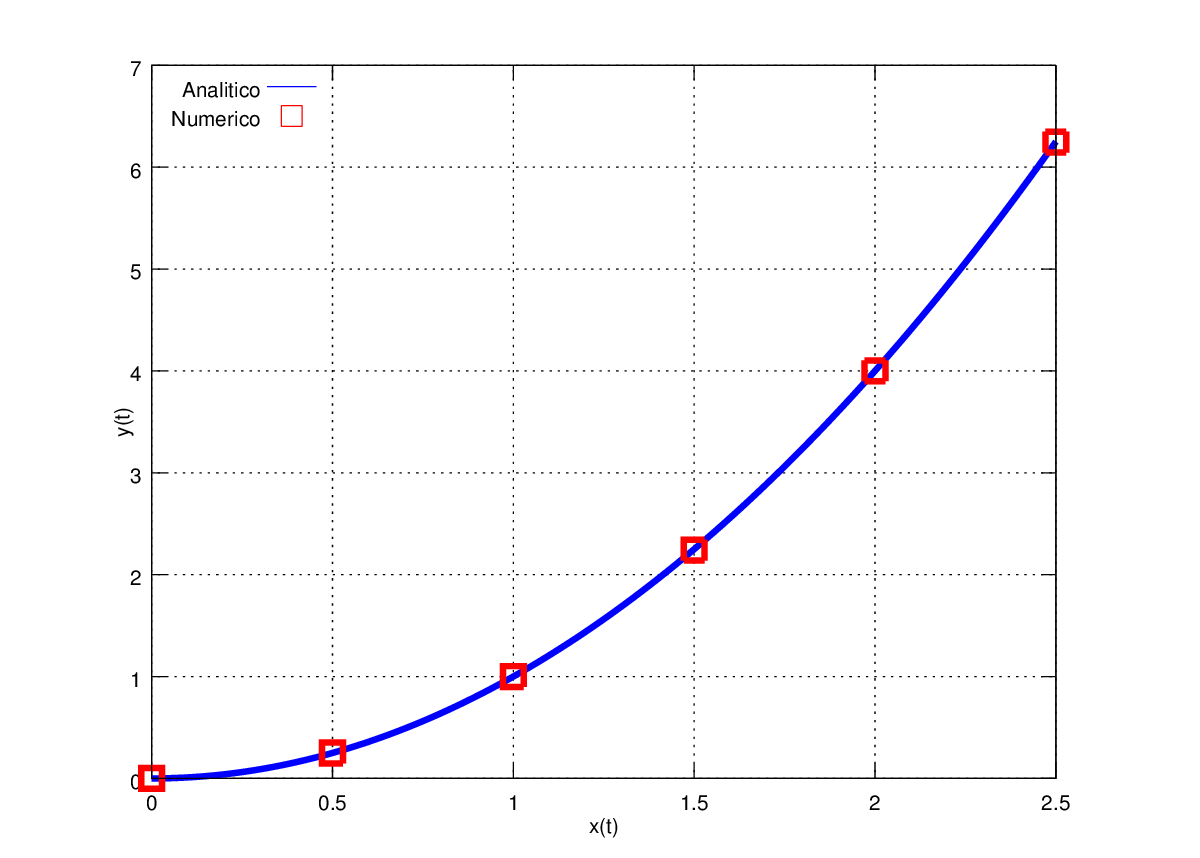
\includegraphics[width=\textwidth]{Figuras/capitulo_2/x_vs_y}
    \caption{Tom and Jerry}
    \label{fig:TomJerry}   
  \end{subfigure}             
  \begin{subfigure}[b]{0.3\textwidth}
    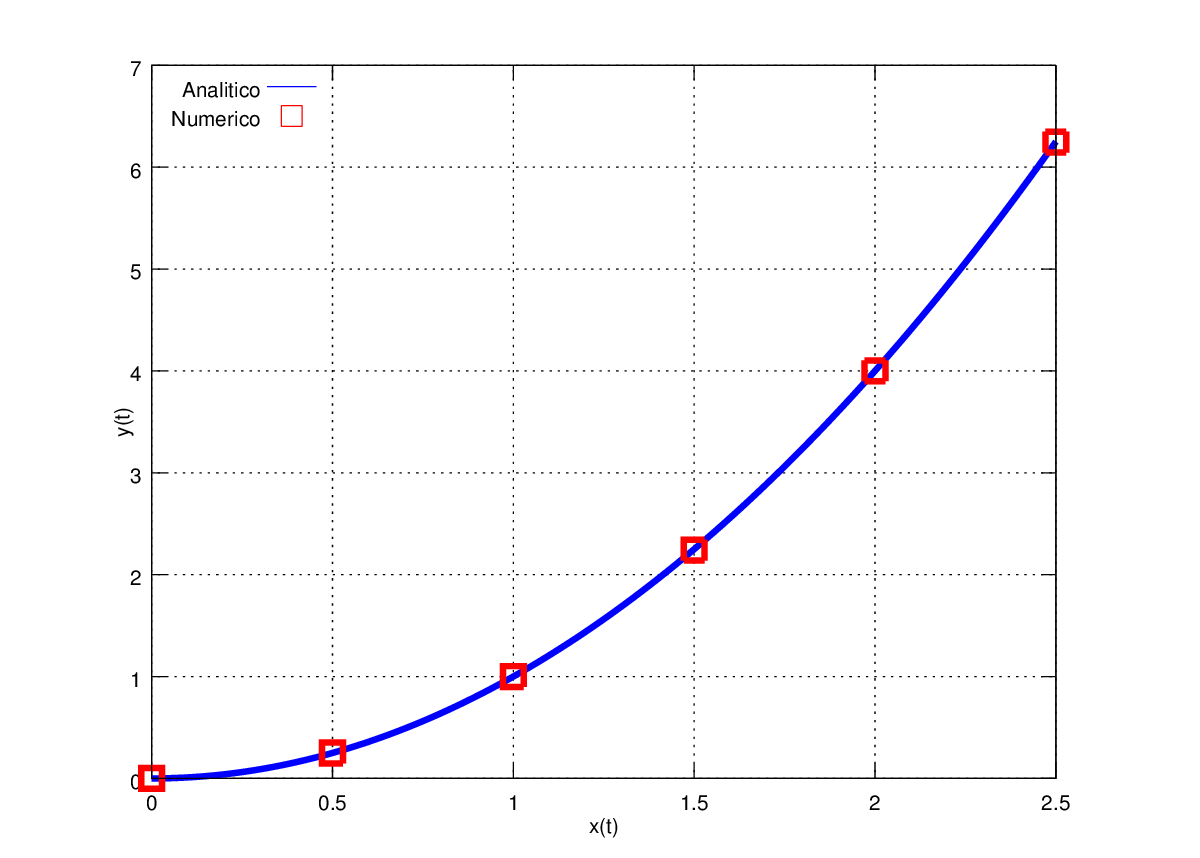
\includegraphics[width=\textwidth]{Figuras/capitulo_2/x_vs_y}
    \caption{Wall-E}
    \label{fig:WallE}
  \end{subfigure}             
  \begin{subfigure}[b]{0.3\textwidth}
    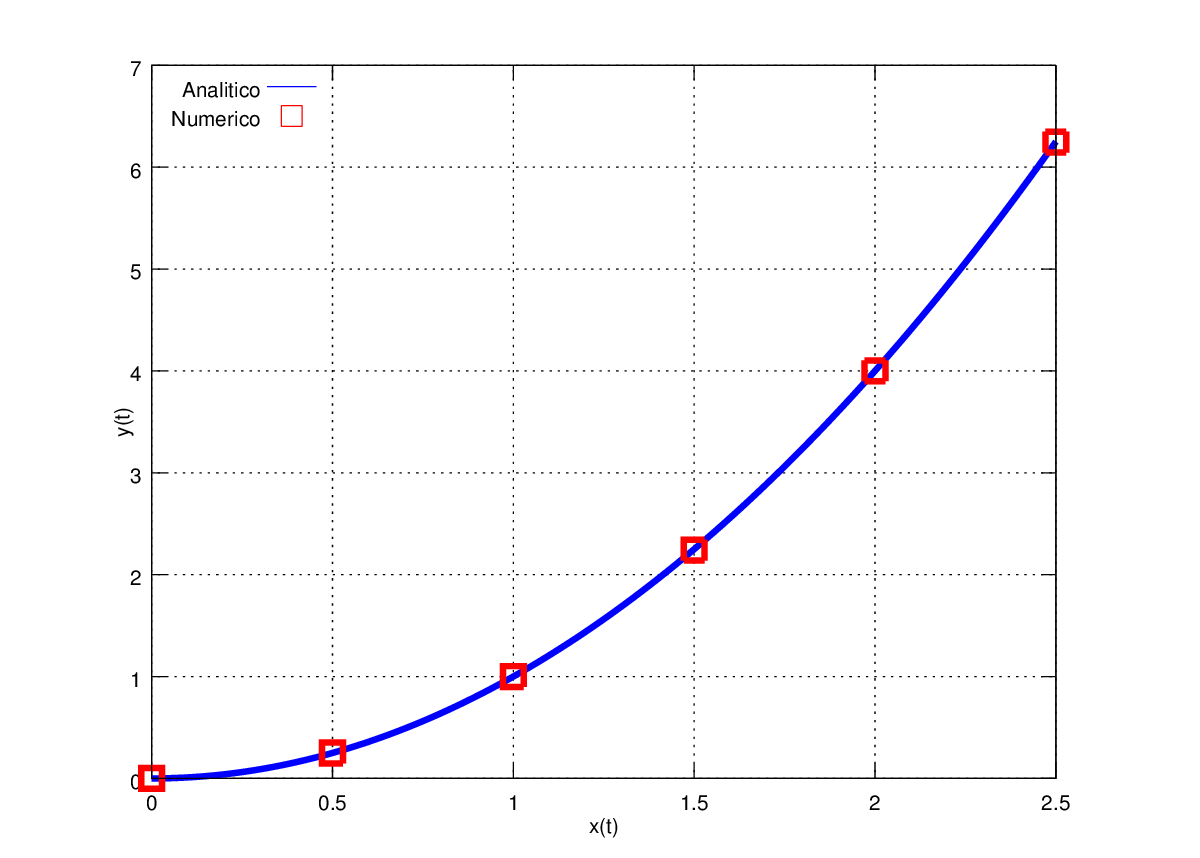
\includegraphics[width=\textwidth]{Figuras/capitulo_2/x_vs_y}
    \caption{Minions}
    \label{fig:Minnion}
  \end{subfigure}
  \caption{Best Animations}
  \label{fig:animations}
\end{figure}


	%!TEX root = ../tesis.tex

\chapter{Tercer capítulo}

\section{Primer sección}
Contenido de la sección \dots \footnote{Una nota al pie.}

Dentro del material bibliográfico se referencia aquí unos pocos a modo de ejemplo, estando los demás incluidos en la guía, como ser: \cite{book-example}, \cite{techreport-example} y \cite{article-example}.

\begin{table}[h]
	\caption{Una tabla mal formateada.}
	\centering
	\label{table:bad_table}
	\begin{tabular}{|l|c|c|c|c|}
	\hline & \multicolumn{2}{c}{Species I} & \multicolumn{2}{c|}{Species II} \\ 
	\hline  Dental measurement  & mean & SD  & mean & SD  \\ \hline 
	\hline	I1MD & 6.23 & 0.91 & 5.2  & 0.7  \\
	\hline 	I1LL & 7.48 & 0.56 & 8.7  & 0.71 \\
	\hline 	I2MD & 3.99 & 0.63 & 4.22 & 0.54 \\
	\hline 	I2LL & 6.81 & 0.02 & 6.66 & 0.01 \\
	\hline 	CMD & 13.47 & 0.09 & 10.55 & 0.05 \\
	\hline 	CBL & 11.88 & 0.05 & 13.11 & 0.04\\ 
	\hline 
	\end{tabular}
\end{table}

\begin{table}[h]
	\caption{Una tabla bien formateada.}
	\centering
	\label{table:good_table}
	\begin{tabular}{l c c c c}
	\toprule
	\multirow{2}{*}{Dental measurement} & \multicolumn{2}{c}{Species I} & \multicolumn{2}{c}{Species II} \\ 
	\cmidrule{2-5}  & mean & SD  & mean & SD  \\ 
	\midrule
	I1MD & 6.23 & 0.91 & 5.2  & 0.7  \\
	I1LL & 7.48 & 0.56 & 8.7  & 0.71 \\	
	I2MD & 3.99 & 0.63 & 4.22 & 0.54 \\	
	I2LL & 6.81 & 0.02 & 6.66 & 0.01 \\	
	CMD & 13.47 & 0.09 & 10.55 & 0.05 \\	
	CBL & 11.88 & 0.05 & 13.11 & 0.04\\ 
	\bottomrule
	\end{tabular}
\end{table}

		
	% Back Matter - NO comentar
	\backmatter
	
	% ***************************** Index ******************************
	\printthesisindex % Índice alfabético, opcional.
	% Apéndices
	\begin{appendices} 
		\chapter{Primer apéndice} \label{Ape1}

Este es el primer apéndice.


		\chapter{Segundo} \label{Ape2}

\section{Sección del apéndice}
Este es el segundo apéndice.
\begin{equation}
	E = m\cdot c^2
\end{equation}

	\end{appendices}
	% Bibliografía	
	\printbibliography[heading=bibintoc]	

\end{document}
